% !TeX spellcheck = fr_CH

% TODO: Replace scan images with clean text where possible

\documentclass[a4paper, 10pt]{report}

\usepackage[french]{babel}
\usepackage[T1]{fontenc}

\usepackage{amsmath, amssymb, amsfonts}

\usepackage{hyperref}
\usepackage{geometry}

\usepackage{xcolor}
\usepackage{graphicx}

\usepackage{fancyhdr}
\usepackage{lastpage}

\usepackage{enumitem}

\geometry{
	a4paper,
	left=25mm,
	right=25mm,
	top=35mm,
	bottom=25mm,
	headsep=5mm,
	headheight=20mm,
}

\definecolor{solution}{HTML}{E5E4E2}
\providecommand{\abs}[1]{\lvert#1\rvert}
\providecommand{\norm}[1]{\lVert#1\rVert}

\begin{document}
	
	\renewcommand{\headrule}{%
		\vspace{-4pt}\hrulefill
		\raisebox{-6.8pt}{\ 
\includegraphics[height=5mm]{../../icon.png}}
		\hrulefill
		}	
	\pagestyle{fancy}
	\fancyhf{}
	
	\fancyhead[L]{\small \slshape Automne 2024}
	\fancyhead[C]{\Large \bfseries Analyse I - Série 01}
	\fancyhead[R]{\small Buff Mathias}
	\fancyfoot[L]{
		\small Source files available at:
		\href{https://github.com/MathiasBuff/bsc-math}
		{github.com/MathiasBuff/bsc-math}
	}
	\fancyfoot[R]{
		\small Page \thepage
		\hspace{1pt} /
		\pageref*{LastPage}
	}
	
	\vspace{5mm}
	\noindent
	\textbf{Exercice 1.} Quelle est la contraposée des implications
	suivantes ? Même question avec la négation.
	%
	\begin{enumerate}[label=(\roman*)]
		\item Si $x > 0$, alors $f(x) \leq 0$.
		\item Si $ab = 0$, alors $(a = 0$ ou $b = 0)$.
	\end{enumerate}
	
	\colorbox{solution}
	{
		\begin{minipage}{0.9\textwidth}
			\begin{enumerate}[label=(\roman*)]
				\item Contraposée : Si $f(x) > 0$, alors $x \leq 0$.\\
					Négation : $(x > 0)$ et $(f(x) >0)$.
				\item Contraposée : Si $(a \neq 0$ et $b \neq 0)$, alors $ab \neq 0$.\\
				Négation : $(ab = 0)$ et $(a \neq 0$ et $b \neq 0)$.
			\end{enumerate}
		\end{minipage}
	}
		
	\vspace{5mm}
	\noindent
	\textbf{Exercice 2.} Expliquer verbalement ce que signifient les
	assertions suivantes et écrire leur négation.
	%
	\begin{enumerate}[label=(\roman*)]
		\item $\forall x \in \mathbb{R}, x^2 < 0$.
		%
		\item $\forall x,y \in \mathbb{Q}, [x < y \implies
			\exists z \in \mathbb{Q}, x < z < y]$.
		%
		\item $\forall A \in \mathbb{R}, \exists n \in \mathbb{N},
			n > A$.
		%
		\item $\forall n \in \mathbb{N}, \exists p \geq n,
			\forall r \mathbb{N}, \forall s \mathbb{N},
			[p = rs \implies (r = 1) \lor (s = 1)]$.
	\end{enumerate}
	
	\colorbox{solution}
	{
		\begin{minipage}{0.9\textwidth}
			\begin{enumerate}[label=(\roman*)]
				\item "Le carré d'un nombre réel est négatif."\\
				Négation : $\exists x \in \mathbb{R}, x^2 \geq 0$.
				%
				\item "On peut trouver un nombre rationnel entre
				chaque paire de nombres rationnels distincts."\\
				\textit{("$\mathbb{Q}$ est dense." ?)}\\
				Négation : $\exists x,y \in \mathbb{Q},
					[x < y \land (\forall z \in \mathbb{Q},
					z < x \land y < z)]$.
				%
				\item "Il existe des entiers naturels arbitrairement
				grands."\\
				Négation : $\exists A \in \mathbb{R},
					\forall n \in \mathbb{N}, n \leq A$
				%
				\item "Il existe une infinité de nombres premiers."\\
				Négation : $\exists n \in \mathbb{N}, \forall p \geq n,
					\exists r \in \mathbb{N}, \exists s \in \mathbb{N},
					[(p = rs) \land (r \neq 1) \land (s \neq 1)]$
			\end{enumerate}
		\end{minipage}
	}
	
	\vspace{5mm}
	\noindent
	\textbf{Exercice 3.} Écrire la négation des assertions suivantes.
	%
	\begin{enumerate}[label=(\roman*)]
		\item $\forall x,y \in E, xy = yx$.
		%
		\item $\exists x \in E, \forall y \in E, xy = yx$.
		%
		\item $\forall a,b \in A, [ab = 0 \implies
			(a = 0) \lor (b = 0)]$.
		%
		\item $\forall x \in \mathbb{R}, \forall y \in \mathbb{R},
			[x < y \implies f(x) < f(y)]$ (où $f$ est une fonction
			de $\mathbb{R}$ dans $\mathbb{R}$).
		%
		\item $\forall \epsilon > 0, \exists N \in \mathbb{N},
			[n \geq N \implies \abs{u_n - \ell} < \epsilon]$
			(où $(u_n)$ est une suite réelle et $\ell \in \mathbb{R}$).
		%
		\item $\exists \ell \in \mathbb{R}, \forall \epsilon > 0,
			\exists N \in \mathbb{N}, [n \geq N \implies
			\abs{u_n - \ell} < \epsilon]$
			(où $(u_n)$ est une suite réelle).
		%
	\end{enumerate}
	
	\colorbox{solution}
	{
		\begin{minipage}{0.9\textwidth}
			\begin{enumerate}[label=(\roman*)]
				\item $\neg[
				\forall x,y \in E,
				xy = yx
				]
				\iff
				\exists x,y \in E,
				xy \neq yx$.
				%
				\item $\neg[
				\exists x \in E,
				\forall y \in E,
				xy = yx
				]
				\iff
				\forall x \in E,
				\exists y \in E,
				xy \neq yx
				$.
				%
				\item $\neg[
				\forall a,b \in A,
				[ab = 0 \implies (a = 0) \lor (b = 0)]
				]
				\iff
				\exists a,b \in A,
				[ab = 0 \land (a \neq 0) \land (b \neq 0)]
				$.
				%
				\item $\neg[
				\forall x \in \mathbb{R},
				\forall y \in \mathbb{R},
				[x < y \implies f(x) < f(y)]
				]
				\iff
				\exists x \in \mathbb{R},
				\exists y \in \mathbb{R},
				[x < y \land f(x) \geq f(y)]
				$
				%
				\item $\neg[
				\forall \epsilon > 0,
				\exists N \in \mathbb{N},
				[n \geq N \implies \abs{u_n - \ell} < \epsilon]
				]
				\iff
				\exists \epsilon > 0,
				\forall N \in \mathbb{N},
				[n \geq N \land \abs{u_n - \ell} \geq \epsilon]
				$
				%
				\item $\neg[
				\exists \ell \in \mathbb{R},
				\forall \epsilon > 0,
				\exists N \in \mathbb{N},
				[n \geq N \implies \abs{u_n - \ell} < \epsilon]
				]\\
				\iff
				\forall \ell \in \mathbb{R},
				\exists \epsilon > 0,
				\forall N \in \mathbb{N},
				[n \geq N \land \abs{u_n - \ell} \geq \epsilon]
				$
				%
			\end{enumerate}
		\end{minipage}
	}
		
	\vspace{5mm}
	\noindent
	\textbf{Exercice 4.} Soient $E, F$ et $G$ trois ensembles. Montrer
	que	si $E \subset F$ et $F \subset G$, alors $E \subset G$.
	
	\colorbox{solution}
	{
		\begin{minipage}{0.9\textwidth}
			Soit $x \in E$. Puisque $E \subset F$, alors $x \in F$.
			De plus, comme $F \subset G, x \in G$.\\
			Donc, $[\forall x \in E, 
			(E \subset F) \land (F \subset G)
			\implies
			x \in G]
			\iff
			E \subset G$.
		\end{minipage}
	}
		
	\newpage
	
	\fancyhf{}
	\renewcommand{\headrule}
	{\rule{\textwidth}{0pt}}
	\fancyfoot[R]{
		\small Page \thepage
		\hspace{1pt} /
		\pageref*{LastPage}
	}
	
	\noindent
	\textbf{Exercice 5.} Soient $A, B$ et $C$ trois ensembles.
	%
	\begin{enumerate}[label=(\roman*)]
		\item Montrer que $A = B \iff (A \cap B = A \cup B)$.
		
		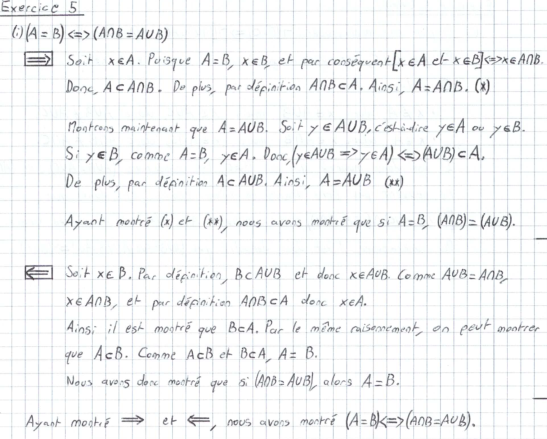
\includegraphics{ex05-1.png}
		
		\newpage
		\item Montrer que $A = B \iff
			(\mathcal{P}(A) = \mathcal{P}(B))$.
		
		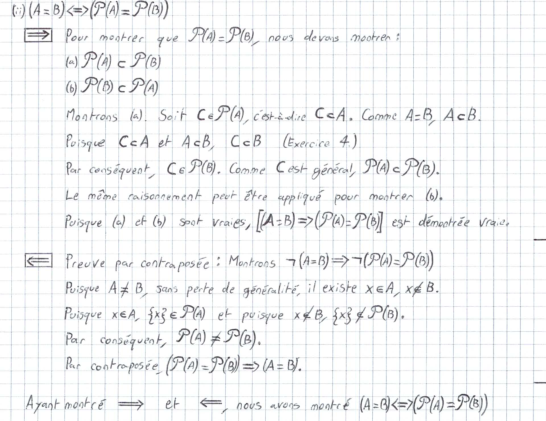
\includegraphics{ex05-2.png}
		
		\item Montrer que $(A \cup B = A \cup C) \land
			(A \cap B = A \cap C) \implies (B = C)$.
		
		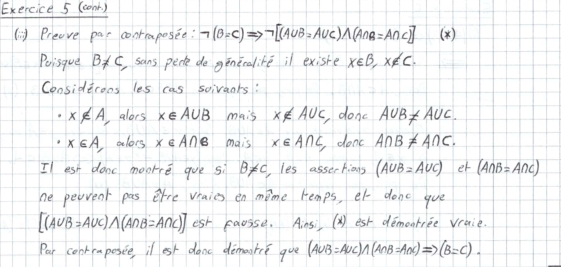
\includegraphics{ex05-3.png}
		
	\end{enumerate}
	
	\newpage
	
	\noindent
	\textbf{Exercice 6.} Dites si les assertions suivantes sont
	VRAIES ou FAUSSES.
	%
	\begin{enumerate}[label=(\roman*)]
		\item $\mathbb{N} \in \mathbb{Z}$.
		%
		\item $\mathbb{N} \subset \mathbb{Z}$.
		%
		\item $\emptyset \in \mathbb{N}$.
		%
		\item $\emptyset \subset \mathbb{N}$.
		%
		\item $\{1,2\} \in \mathcal{P}(\{1,2,3\})$.
		%
		\item $\{1,2\} \subset \mathcal{P}(\{1,2,3\})$.
		%
		\item $\{\{1\}\} \subset \mathcal{P}(\{1,2,3\})$.
		%
	\end{enumerate}
	
	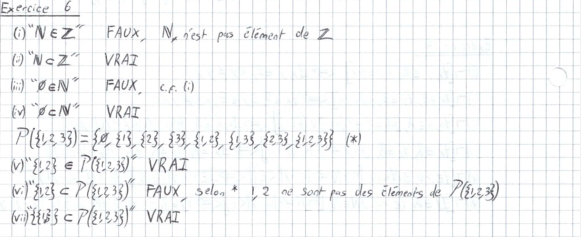
\includegraphics{ex06.png}
	
	\vspace{5mm}
	\noindent
	\textbf{Exercice 7.} Considérons les sous-ensembles de $\mathbb{N}$
	%
	\[
		A = \{1,2,3,4,5,6,7\}, \quad B = \{1,3,5,7\}, \quad
			C = \{2,4,6\}, \quad D = \{3,6\}.
	\]
	%
	\begin{enumerate}[label=(\roman*)]
		\item Déterminer $B \cap D$ et $C \cap D$.
		%
		\item Déterminer $B \cup D$ et $C \cup D$. L'une de
		ces deux unions est-elle disjointe ?
		%
		\item Déterminer les complémentaires dans $A$ de $B, C$ et $D$.
		%
	\end{enumerate}
	
	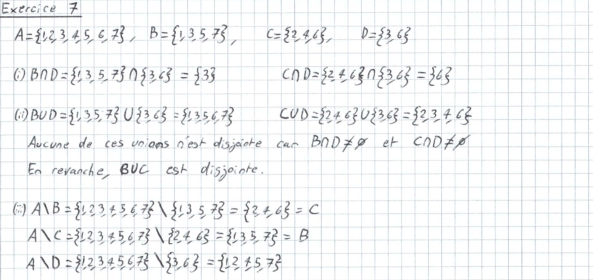
\includegraphics{ex07.png}
	
\end{document}